\section{Einführung}

\subsection{Prinzip}

Die FM Synthese ist eine für die Musikwelt sehr wichtige Anwendung der Frequenzmodulation, welche bereits aus der Nachrichtentechnik bekannt ist. Generell wird dabei die Frequenz eines Trägersignals durch ein weiteres Modulationssignal verändert, die Amplitude bleibt jedoch unangetastet. In der Nachrichtentechnik können durch die unterschiedlichen Frequenzen im modulierten Trägersignal dadurch Informationen übertragen werden. 

Die momentane Amplitude des modulierten Signales lässt sich durch folgende Formel beschreiben:

\[
\epsilon = A*\sin(\alpha*t + I*\sin(\beta*t)) 
\]

Bei der äußeren Sinusfunktion handelt es sich um das Trägersignal, welches in seiner Frequenz durch das Modulationssignal (Innerer Sinus) moduliert wird.


Die folgende Grafik veranschaulicht die Frequenzmodulation eines Signals durch ein zweites Signal:

\begin{figure} [ht]
\centering
  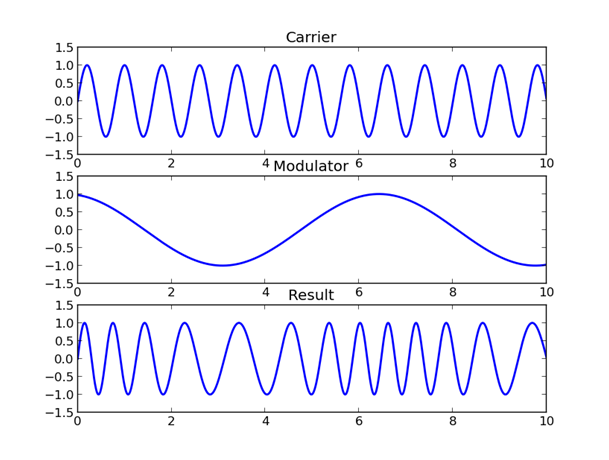
\includegraphics[width=0.95\textwidth]{Signalbeispiel.png}
\caption{Vergleich Träger/Modulator}
Quelle: Test
\end{figure}

Wie man gut erkennen kann, wird die Frequenz des Trägers bei hoher Amplitude des Modulators größer, bei negativer Amplitude dagegen kleiner. Ist die Amplitude des Modulator gleich 0, so wird das Trägersignal nicht moduliert.

Die Frequenzmodulationssynthese ist in ihren Grundzügen recht einfach zu verstehen und man kann mit geringem  Aufwand bereits sehr komplexe, wenn auch oft unkontrollierbare, Signale mit komplexen Klangspektren (bzw. Frequenzspektren) erzeugen. Wie sich im Folgenden jedoch noch herausstellen wird, ist es dagegen sehr schwierig und erfordert viel Zeit und Aufwand, durch die FM-Synthese gezielt Signale zu erzeugen und diese zu kontrollieren. Eine Möglichkeit zur Erzeugung komplexer Klangspektren ist es, den Modulationsindex innerhalb des Trägersignals zeitabhängig zu machen. Dieses Verfahren wird im Kapitel X näher erläutert.

Praktisch gesehen kann die Frequenzmodulations-Synthese dazu verwendet werden, um zum Einen Klangbilder echter Instrumente digital nachzubilden, jedoch auch, um ganz neue Töne zu erzeugen, die so in der realen Welt nicht vorkommen. Im Folgenden sind einige Beispiele von durch FM-Synthese erzeugten Signalen zu sehen.

\subsection{Beispiel (Sound \& Visualisierung)}
\subsection{Geschichte (auch GS1)}